\documentclass[12pt]{article}

\usepackage{sbc-template}

\usepackage[brazil]{babel}
\usepackage[utf8]{inputenc}

\usepackage[alf]{abntex2cite}
\usepackage{graphicx}
\usepackage{float}
\usepackage{soul}
\usepackage{color}
\newcommand{\hilight}[1]{\colorbox{yellow}{#1}}

\graphicspath{{\main/imagens/}{imagens/}}

\AtBeginEnvironment{quote}{\smaller} % Step font down one size relative to current font.

\sloppy

\title{\normalfont{Desenvolvimento de Documentação e Implementação de Sistema de Informação
para Auxílio na Aprendizagem de Qualidade de Software}}

\author{Vinícius B. Bruscagini\inst{1}, Carlos R. S. Júnior\inst{1}}

\address{Instituto Federal de Educação, Ciência e Tecnologia do Estado de São Paulo\\Campus Hortolândia (IFSP-HTO)
\email{vinicius.bruscagini@aluno.ifsp.edu.br, carlos.rsantos@ifsp.edu.br}}

\begin{document}

\maketitle

\begin{abstract}
  This paper has the objective to create an App using famous technologies and tools
  avaliable on the market. Applying software quality and project management concepts.
  A documentation covering all the aspects of the system will be released to help students
  and developers understand these concepts in a practical way.
\end{abstract}

\begin{resumo}
  Este trabalho possui o objetivo de criar um sistema de informação utilizando tecnologias e ferramentas
  famosas no mercado, aplicando conceitos de qualidade de software e gerenciamento de projetos.
  Será disponibilizado um material que documentará todos os aspectos desse sistema, de forma a ajudar
  estudantes e desenvolvidores a entenderem como funcionam conceitos de qualidade de software na prática.
\end{resumo}

\section{Introdução}

A área de TI, incluindo desenvolvimento de software, é uma área que evoluiu muito nas ultimas
décadas~\cite{Pacheco10} e continua evoluindo rapidamente até hoje. Novas Tecnologias e ferramentas
surgem em rítmo acelerado e muitas delas ganham popularidade, demandando assim, novas
habilidades para os profissionais de TI\@. Com essa evolução, os cursos oferecidos nessa área não conseguem
oferecer disciplinas sobre tecnologias usadas no mercado. O ensino, então, não propicia o aprendizado
suficiente para os profissionais de TI, fazendo com que muitos desses busquem cursos ou certificações para
aprimorar seus conhecimentos.~\cite{macedo09}. Além disso, de acordo com uma pesquisa realizada por
~\cite{wei08} os alunos de cursos de Engenharia de Software se preocupam em possuir um aprendizado
voltado para prática e sempre ter convivência com conceitos e métodos importantes para o mercado de trabalho.

Baseando-se nessas questões, a produção desse trabalho tem a proposta de desenvolver
um sistema com tecnologias e ferramentas populares que possuem demanda por profissionais,
com o objetivo principal de construir uma documentação
que abrange todos os aspectos desse sistema e que explique com clareza como o software
funciona, quais tecnologias foram usadas e como se deu o seu desenvolvimento.
O código fonte da aplicação e a documentação serão publicados e então esses materiais
poderiam ser consultados por qualquer pessoa, assim ajudando elas a
entenderem alguns conceitos de Desenvolvimento de Software e como se dão suas aplicações na prática.

\section{Fundamentação Teórica}

Para atingirmos um software conforme descrito na seção anterior, precisamos entender
alguns conceitos importantes dessa área.

\subsection{Framework}

Um conceito importante no desenvolvimento de sistemas é o `Framework', de acordo com~\cite{host12} um
framework é como um template que conta com diversas funcionalidades. Ele possui o objetivo principal de
resolver problemas recorrentes no desenvolvimento e acelerar esse processo. O
Projeto Pedagógico do Curso de Análise e Desenvolvimento de Sistemas do IFSP - Campus Hortolândia
contém uma disciplina que ensina o uso de um framework para o desenvolvimento. No entanto, a bibliografia básica
que aborda esse framework é do ano de 2010 e faz uso da tecnologia JSF, que hoje em dia é muito pouco usada.~\cite{webtechsurveyJSF}

% explicar o que é qualidade e arquitetura de "sistema de produção"
\subsection{Qualidade de Software}

A definição de qualidade no contexto da computação nem sempre é um consenso,
existem diferentes terminologias, as quais podem causar problemas para pessoas que não
possuem conhecimento sobre.~\cite{Duarte03}

Um software pode ser considerado de qualidade quando ele atende a todas as necessidades, explicitas
e implícitas para qual ele foi feito.~\cite{Duarte03}

Enquanto ao código, que será o foco do artigo, existem padrões que devem ser seguidos para um código
possuir qualidade. Para isso devemos pontuar que para um código ter qualidade ele deve funcionar, e principalmente,
ser légivel.

\begin{quote}
  ``Muitos programadores iniciantes acham que um bom código é aquele que é correto, ou seja, faz o que tem
  que fazer.''~\cite{Levy04}.
\end{quote}

Um código, para funcionar deve possuir ao menos duas características, ele deve ser \textbf{Correto} e \textbf{Eficiente},
esses pontos são o que fazem um código funcionar. Porém isso não é o suficiente para ser considerado
um código de qualidade. No mundo real, códigos são criados, alterados e revistos, geralmente por diferentes pessoas,
por isso existem duas propriedades adicionais que um código deve possuir, ele deve ser \textbf{Elegante} e \textbf{Testável}
como descritos por~\cite{Levy04}.

Um código elegante e testável dá qualidade ao nosso código pois isso facilita, e muito, sua manutenção.

\subsection{Controle de Versão}

Controle de versão é a prática de rastrear e gerenciar mudanças no código do software~\cite{attlasianGit}.
Essas ferramentas gerenciam o código fonte de projetos ao longo do tempo, e possuem informações detalhadas
de todas as modificações que foram realizadas em todos os arquivos do código fonte.
Alguns dos benefícios que essas ferramentas proporcionam são rastreabilidade (quem fez o quê),
ajudam na resolução de conflitos e aceleram o desenvolvimento. A ferramenta mais famosa para controle de
versão atualmente é o Git.

\subsubsection{Git}

O Git é a ferramenta mais usada para controle de versão. De acordo com seu website, ele
funciona com o conceito de \textit{commits} e \textit{branches}, em que um \textit{commit}
é uma alteração realizada no código, e uma \textit{branch} é uma ramificação do código, elas são
exemplificadas na figura~\ref{fig:git-branches}.

\begin{figure}[H]
  \centering
  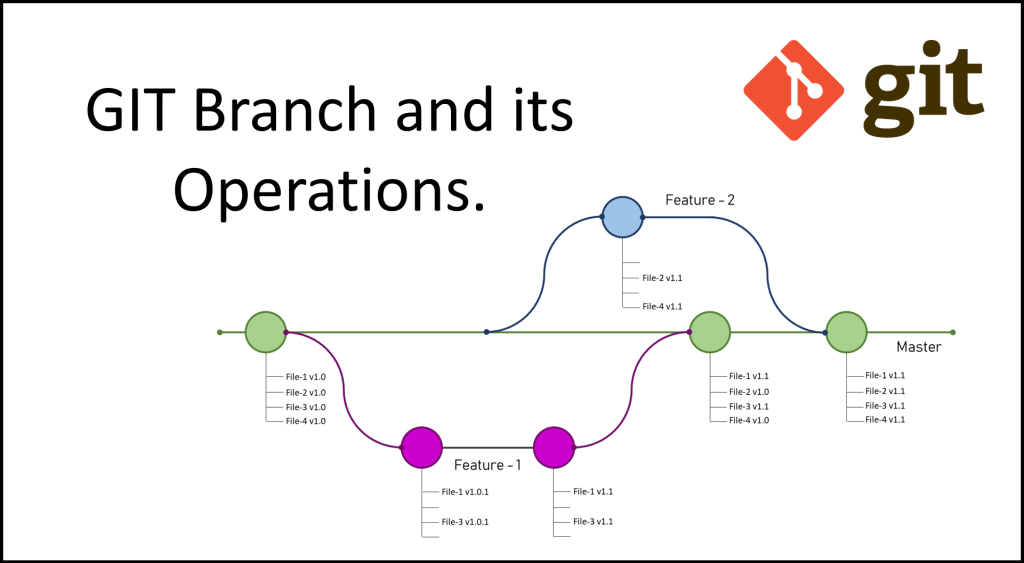
\includegraphics[width=1\textwidth]{git/git-branches.png}
  \caption{Exemplos de branches em um repositório Git}\label{fig:git-branches}
\end{figure}

A figura~\ref{fig:git-branches} mostra três \textit{branches} de um repositório,
uma chamada \textit{master}, outra de \textit{Feature 1} e uma outra chamada \textit{Feature 2}.

Durante o desenvolvimento de um software, essas ramificações acontecem frequentemente. Nesse exemplo,
há duas ramificações que foram criadas para desenvolver uma funcionalidade no software, também chamado de \textit{feature},
ou seja, a partir de uma branch principal \textit{Master}, foram criadas duas \textit{branches} onde o desenvolvimento
de uma funcionalidade foi feita, e ao final desse desenvolvimento, o código feito nessa \textit{branch} foi
unido junto com a \textit{branch} principal.

Com o Git instalado em um computador podemos usar o comando \textbf{git} para realizarmos operações.
Um típico fluxo de um desenvolvimento usando Git é mostrado na figura~\ref{fig:git-lifecycle}.

\begin{figure}[H]
  \centering
  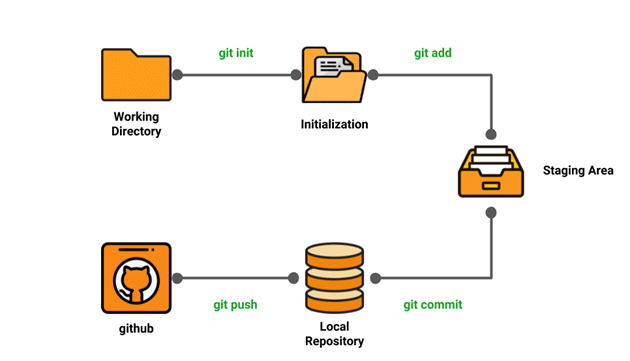
\includegraphics[width=.8\textwidth]{git/git-lifecycle.png}
  \caption{Típico ciclo de desenvolvimento com Git}\label{fig:git-lifecycle}
\end{figure}

O Git funciona em repositórios, que é uma pasta onde estão os arquivos de código de um sistema,
a partir desse repositório, modificações são feitas no código, as quais são adicionadas em um \textit{commit}
e esse \textit{commit} é enviado para um repositório remoto, onde outras pessoas da equipe podem obter as modificações feitas.

\subsection{Documentação de Software}

De acordo com~\cite{Forward02softwaredocumentation}, a documentação de um software é qualquer
artefato que possui como finalidade informar sobre ele, em qualquer um de seus aspectos.

~\cite{Coelho_2009} nos mostra dois tipos de documentações, são esses tipos

\begin{itemize}
	\item Documentação Técnica
	\item Documentação de Uso
\end{itemize}

As documentações técnicas de um sistema é toda aquela documentação voltada ao desenvolvedor e é
ela que informa como o sistema funciona internamente, sua arquitetura, tecnologias usadas e outros detalhes de implementação.

As documentações de uso são documentos que são focados nos usuários finais do sistema e as vezes também para administratores do sistema,
essas documentações geralmente mostram como usar o sistema.

Ambos os tipos de documentações são muito importantes no processo de desenvolvimento e entrega de softwares. A falta ou
baixo nível de qualidade de documentações atrapalham na compreensão do sistema e podem apresentar
riscos para sua manutenção~\cite{deinvestigaccao}.

\subsection{Metodologias Ágeis}

As metodologias ágeis surgiram na década de 80 para melhorar a área de desenvolvimento de software,
que era algo muito rigoroso naquela época, muitos projetos possuiam problemas e as metodologias ágeis foram então
criadas para tentar solucioná-los.~\cite{Santos05}

\subsubsection{Kanban}

O Kanban é uma metodologia que possui cinco princípios de acordo com~\cite{Agile06}
\begin{itemize}
  \item Visualização
  \item Limitar o desenvolvimento em progresso
  \item Medir e gerenciar a sequencia de trabalho
  \item Explicitar o processo
  \item Reconhecimento de oportunidades
\end{itemize}

O Kanban funciona com quadros, onde em cada quadro temos várias seções.
Nessas seções podemos agrupar tarefas.

Em um quadro Kanban podemos agrupar tarefas, definir datas e responsáveis, entre vários outros
detalhes, o que facilita a organização e visão das tarefas do projeto.

Existem várias ferramentas que implementam essa metodologia.
Uma delas é o \emph{GitHub Projects}, que usaremos neste trabalho. É usada para gerenciamento de projetos
com a metodologia Kanban. A interface desse programa é mostrada na Figura~\ref{fig:github-board}.

\begin{figure}[H]
  \centering
  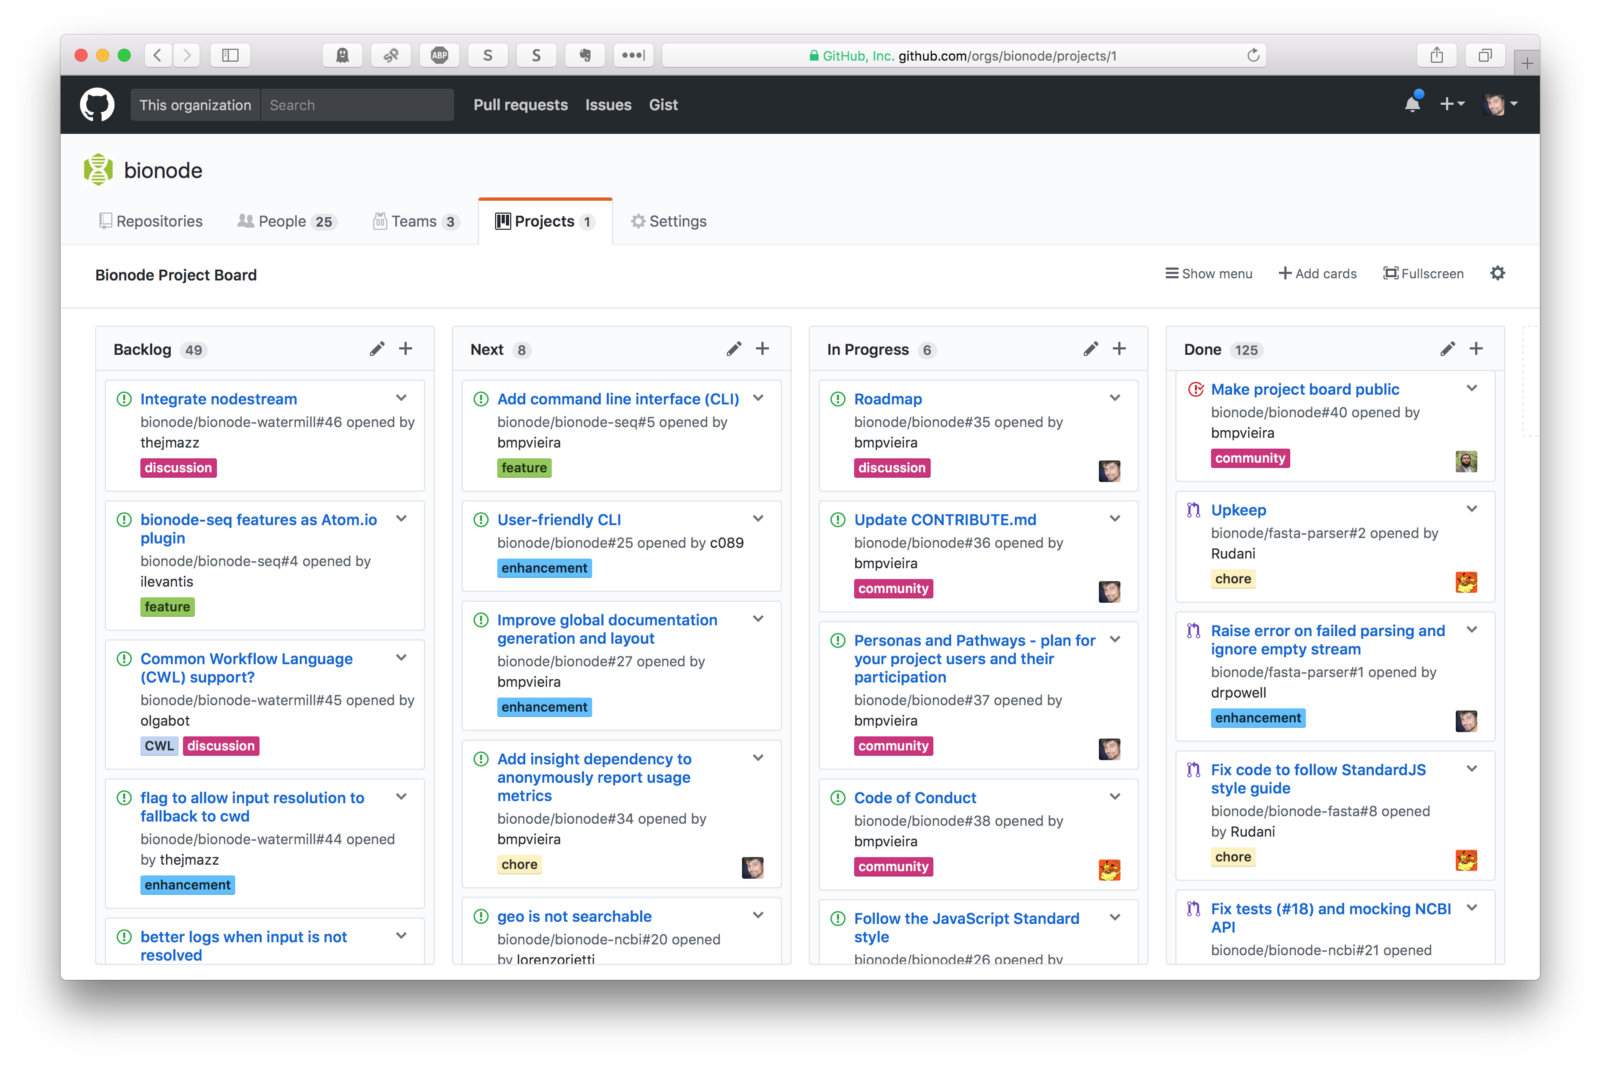
\includegraphics[width=1\textwidth]{github/github-board.png}
  \caption{Tela de um quadro Kanban do \emph{GitHub Projects}}\label{fig:github-board}
\end{figure}


% TODO: Falar de um pouco de Testes unitários aqui

\section{Metodologia}

Para início do desenvolvimento será realizada a definição das tecnologias do sistema, para isso, serão feitas
pesquisas bibliográficas em websites como \textit{GitHub} e \textit{Stackoverflow}. Estes websites
são famosos na área de desenvolvimento, além de que eles podem nos fornecer informações interessantes sobre quais
são as tecnologias mais ativas, mais comentadas e outros dados que podemos usar como base para realizamos
a escolha das tecnologias.

Com a definição das tecnologias, partiremos para a análise e documentação de requisitos do sistema, e a partir
dos requisitos serão criados os diagramas de classe e casos de uso.

Para o desenvolvimento, usaremos os recursos oferecidos pela plataforma GitHub, esses recursos serão

\begin{itemize}
  \item Repositório Git
  \item Quadro Kanban para gerenciamento de projetos
  \item Actions para processos de \textit{Pipelines}
\end{itemize}

\section{Desenvolvimento do Trabalho}

Em Maio de 2021 foi realizada pelo site~\cite{stack11}, uma pesquisa com desenvolvedores de todo o mundo para
coletar dados geográficos, sociais e de uso de tecnologias de seus usuários. Esses dados nos permitem ter
informações importantes sobre o uso de tecnologias em geral. A pesquisa nos dá três conjuntos
de informações relevantes para usarmos no trabalho

\begin{itemize}
  \item Frameworks para Web mais utilizados
  \item Frameworks gerais mais utilizados
  \item Ferramentas para deploy e gerenciamento mais usadas
  \item Banco de Dados mais utilizados
\end{itemize}

Os resultados dessas categorias, entre desenvolvedores profissionais, são exibidos nas
Figuras~\ref{fig:web-frameworks},~\ref{fig:general-frameworks},~\ref{fig:tools} e~\ref{fig:databases}, respectivamente.

\begin{figure}[H]
  \centering
  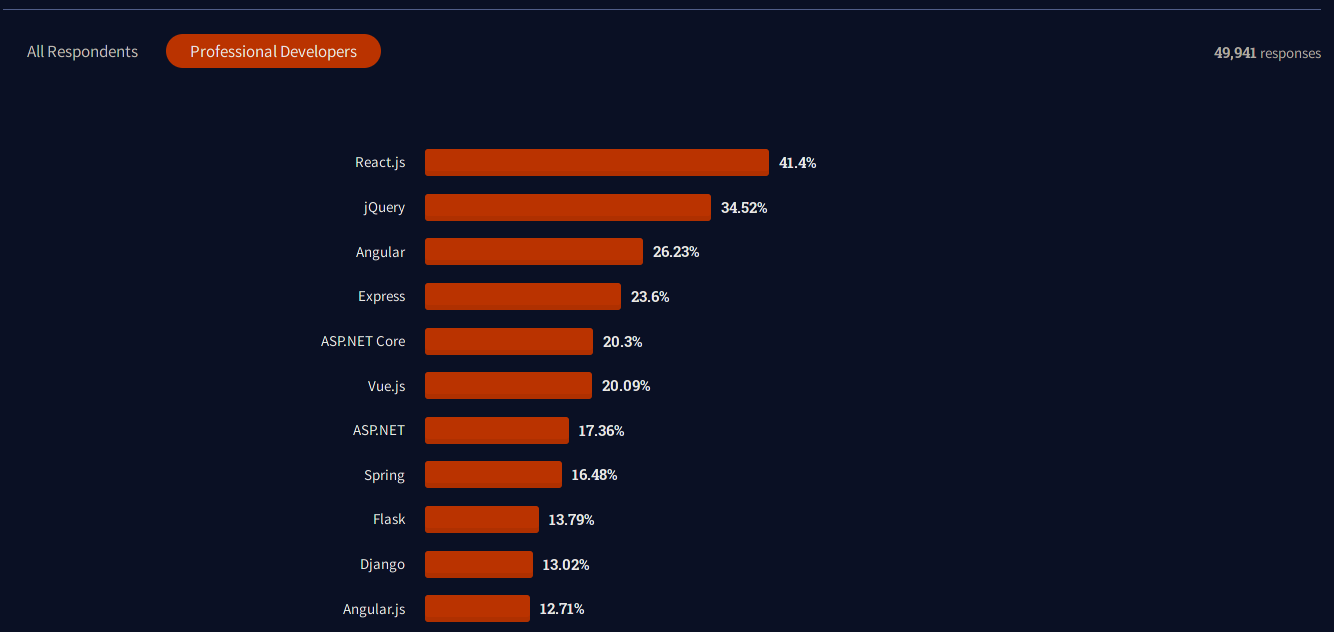
\includegraphics[width=1\textwidth]{stackoverflow/web_frameworks_usage.png}
  \caption{Gráfico mostrando os frameworks Web mais usados}\label{fig:web-frameworks}
\end{figure}

\begin{figure}[H]
  \centering
  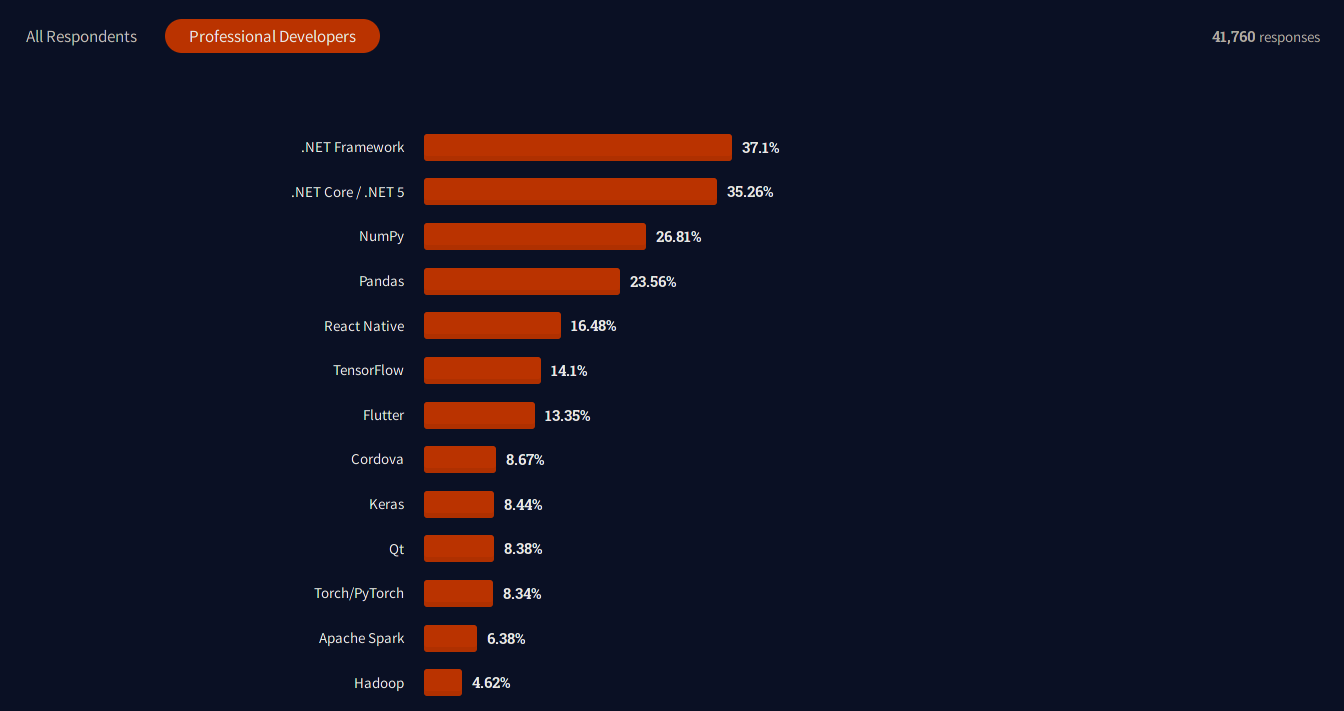
\includegraphics[width=1\textwidth]{stackoverflow/general_framework_usage.png}
  \caption{Gráfico mostrando os frameworks gerais mais usados}\label{fig:general-frameworks}
\end{figure}

\begin{figure}[H]
  \centering
  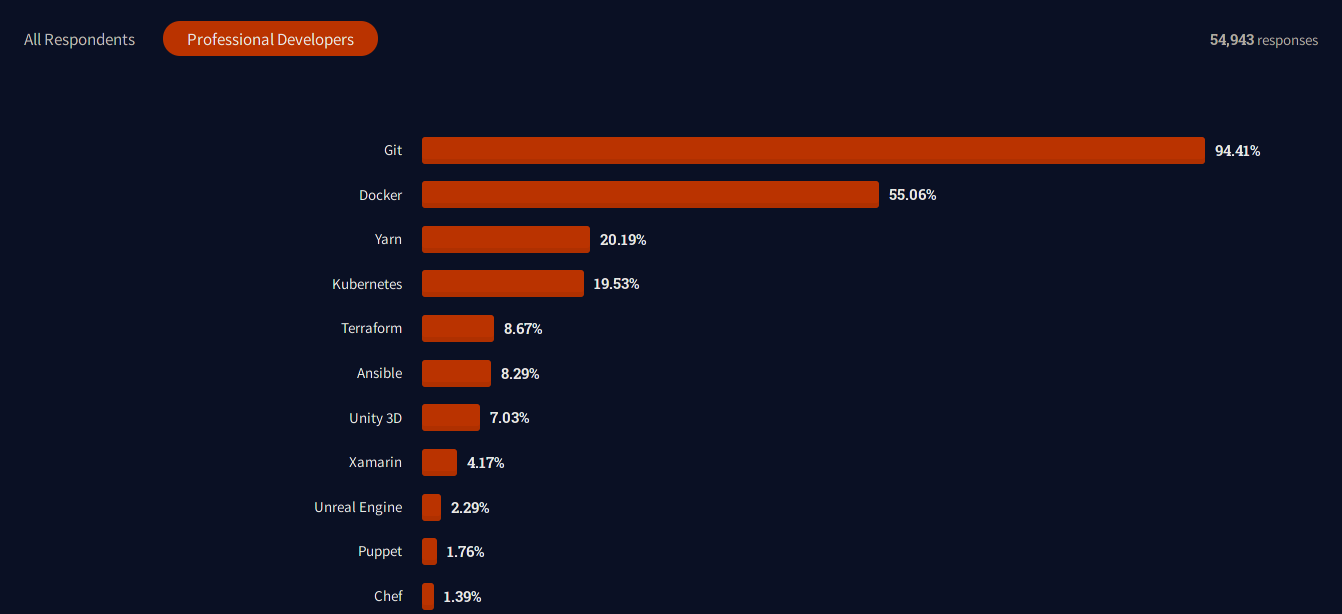
\includegraphics[width=1\textwidth]{stackoverflow/used_tools.png}
  \caption{Gráfico mostrando as ferramentas mais usadas}\label{fig:tools}
\end{figure}

\begin{figure}[H]
  \centering
  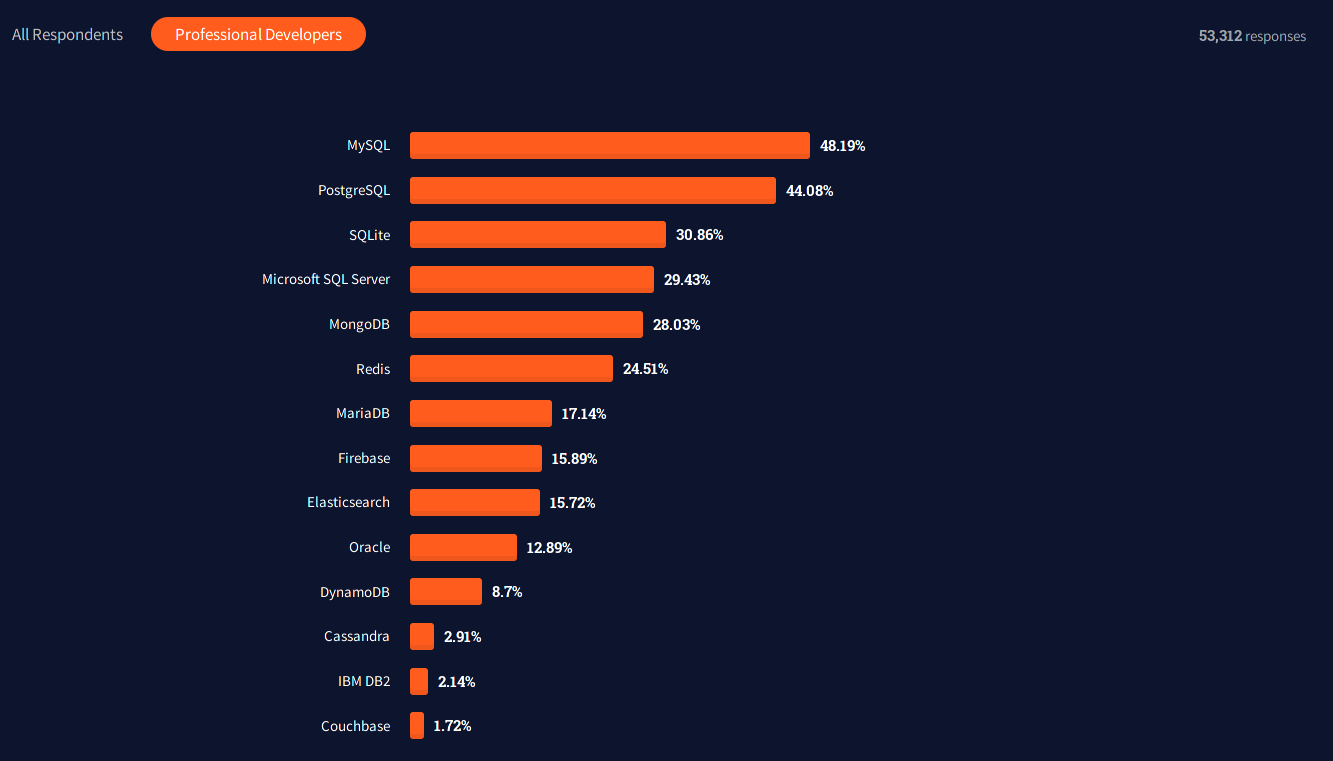
\includegraphics[width=1\textwidth]{stackoverflow/databases.png}
  \caption{Gráfico mostrando os SGBDs mais usados}\label{fig:databases}
\end{figure}

Baseando-se nesses dados de utilização e na experiência do autor em certas tecnologias e ferramentas,
foi optado o uso das tecnologias e arquitetura apresentadas a seguir.

\subsection{Arquitetura}

O sistema terá duas aplicações principais, uma sendo o lado do servidor (Back-End) e outra sendo
a aplicação que será usada pelos usuários (Front-End).

O Back-End será um WebService RESTFul, que será desenvolvido com o ASP.NET Core
junto com a ferramenta de ORM, Entity Framework Core.

o Front-End será uma aplicação Web que será desenvolvida com o Framework Vue.js.

\subsection{WebService}

Um WebService é um serviço que é oferecido e é por onde aplicações se comunicam com o servidor.
WebServices fazem parte da arquitetura orientada a serviços (SOA).

Um tipo de WebService muito utilizado é o REST, que significa
\emph{Representational State Transfer} ele funciona servindo requisições de clientes
para certos serviços. Por exemplo, suponha que um WebService REST tenha uma URL que fornece
informações de funcionários

\begin{verbatim}
  GET http://meuwebservice/funcionarios
\end{verbatim}

GET é o método HTTP usado para requisitar as informações que queremos, então se enviarmos uma requisição
para a URL com o método esperado, o WebService irá responder a requisição com dados em formato JSON com as informações que queremos, por exemplo:

\begin{verbatim}
  [
    {
      "nome": "João",
      "departamento": "Contabilidade"
    },
    {
      "nome": "Bianca",
      "departamento": "Engenharia"
    }
  ]
\end{verbatim}

Um WebService REST pode ter vários URLs, também chamadas de EndPoints, além de obter informações, podemos realizar
diferentes operações em diferentes EndPoints, como inserir um objeto no sistema, por exemplo.

\subsection{ASP.NET Core}

O ASP.NET Core faz parte da família de tecnologias .NET que são desenvolvidas pela Microsoft.
Ele nos permite criar qualquer tipo de aplicação web.

A Plataforma .NET possui uma longa história, por grande parte dessa história, suas
tecnologias foram exclusivas para o sistema operacional Windows. Em 2014 a Microsoft recriou
essa plataforma do zero, hoje toda a plataforma é \textit{open-source} e funciona em qualquer
sistema operacional.

\subsection{Entity Framework Core}

O Entity Framework Core é um framework ORM que é usado em conjunto com o .NET.
Como explicitado por~\cite{ormHibernate}

\begin{quote}
  `Um framework ORM provê uma metodologia e mecanismo
  para sistemas orientados a objetos manterem seus dados em um banco de dados de maneira
  segura, com controle de transações, e tudo isso expressado em código orientado a objeto'.
\end{quote}

De maneira prática, um ORM permite manipularmos entidades em um banco de daddos
sem precisarmos mexer com SQL. Eles geralmente funcionam mapeando as classes
que criamos em nosso código, e com essas informações ele cria o banco de dados já com os relacionamentos
entre as tabelas e tudo mais o que definimos nas classes.

O Entity Framework é o ORM oficial do .NET, possui amplo suporte e uso. Ele será
usado nesse projeto para facilitar a manipulação dos dados no banco de dados.

\subsection{Vue.js}

O Vue é um framework para desenvolvimento de aplicações Web, usando a linguagem JavaScript,
ele nos permite o desenvolvimento de aplicações reativas e possibilita o reuso
de código através de componentes. Abaixo um pequeno código HTML de um arquivo vue

\begin{verbatim}
  <div>
    <p v-if="seen">Agora você me viu</p>
  </div>
\end{verbatim}

Esse trecho de código exibe o texto `Agora você me viu' caso a variável `seen' seja verdadeira.

O Vue nos dá a opção de usar a linguagem TypeScript ao invês do JavaScript, ele possui
várias bibliotecas que melhoram a legibilidade e arquitetura de um componente vue.
Abaixo um código de um componente Vue usando TypeScript

\begin{verbatim}
<template>
  <p>Texto</p>
</template>

<script lang="ts">
import Vue from "vue";
import Component from "vue-class-component";

@Component
export default class About extends Vue {

}
</script>
\end{verbatim}

O Vue possui um ecosistema de bibliotecas adicionais para ajudar no desenvolvimento de aplicações.
Uma dessas bibliotecas é o \textit{Vuetify}, ele fornece para o desenvolvedor componentes para interface
como botões, cards, campos de textos, etc.

\subsection{Gerenciamento}

Durante o desenvolvimento do projeto, serão usadas as funcionalidades da plataforma GitHub, isso inclui
o repositório Git para controle de versão e o quadro Kanban para gerenciamento de Projetos.

\subsection{Definição de Requisitos}

Com o processo e as tecnologias definidas. Agora será decidido o domínio do sistema a ser desenvolvido
e seus requisitos.

Como o foco do trabalho não é o domínio da aplicação, foi optado por copiar o funcionamento de uma aplicação
existente, a aplicação escolhida é o Reddit.

O Reddit, de acordo com seu website é:

\begin{quote}
  `A casa de milhares de comunidades, conversas sem
  limite e interação humana autentica.'
\end{quote}

O Reddit consiste de comunidades que tratam de determinado assunto, nessas comunidades, usuários
podem se inscrever e realizar postagens, as quais outros usuários dessa comunidade virão e podem
dar um voto positivo ou negativo para essa postagem.

Foram criados dois diagramas de casos de uso que representam as funcionalidades esperadas no sistema,
eles são apresentados nas figuras~\ref{fig:welcome_diagram} e~\ref{fig:home_diagram}

%TODO Diagrama está com nome antigo [Simple Forum]

\begin{figure}[H]
    \centering
    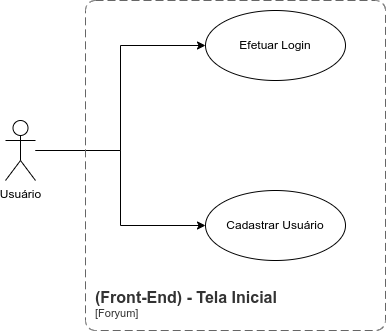
\includegraphics[width=0.7\textwidth]{diagrams/welcome_diagram.png}
    \caption{Diagrama de caso de uso da tela inicial}\label{fig:welcome_diagram}
\end{figure}

\begin{figure}[H]
    \centering
    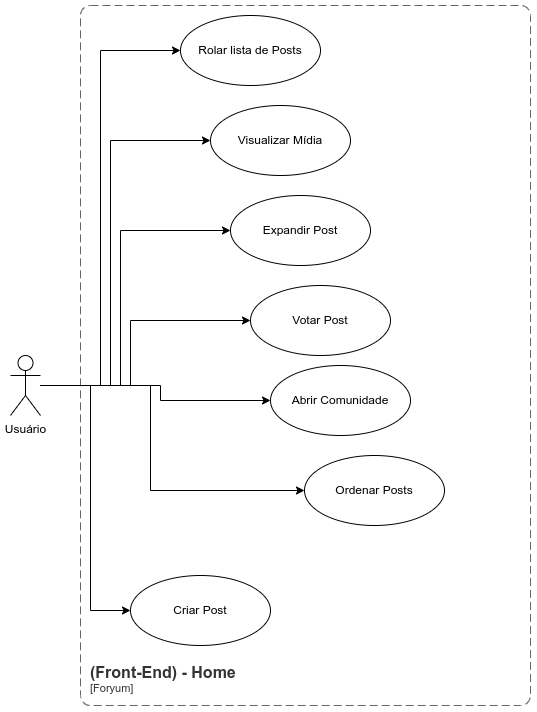
\includegraphics[width=0.7\textwidth]{diagrams/home_diagram.png}
    \caption{Diagrama de caso de uso da tela \textit{home}}\label{fig:home_diagram}
\end{figure}

Junto com os casos de uso foram definidos as propiedades das entidades do sistema
a partir da criação de um diagrama de classe, o diagrama resultante é exibido na figura~\ref{fig:classes_diagram}

\begin{figure}[H]
    \centering
    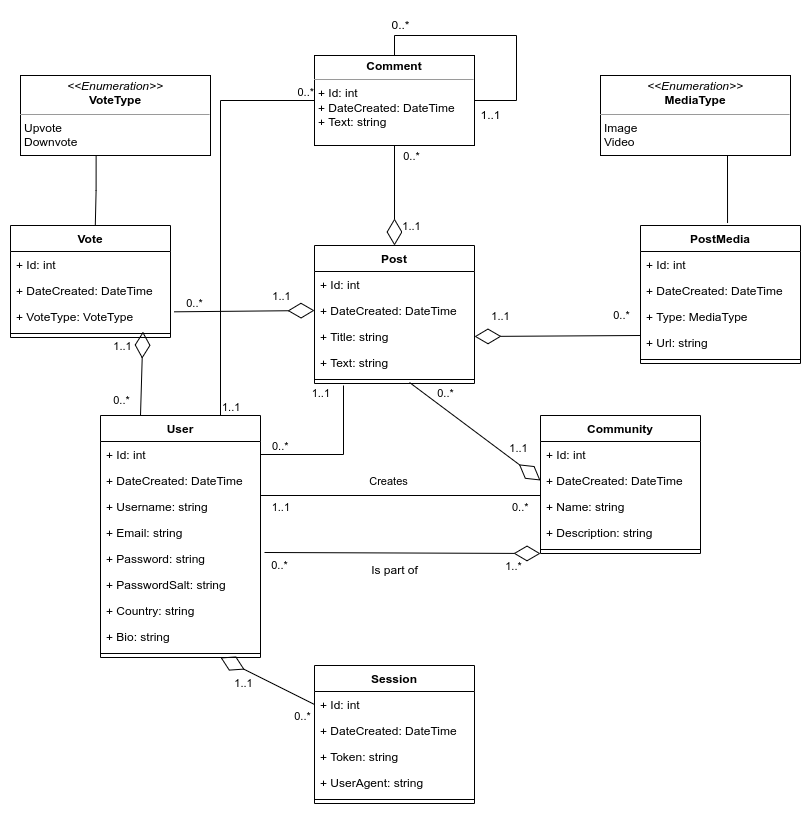
\includegraphics[width=0.8\textwidth]{diagrams/classes_diagram.png}
    \caption{Diagrama de classes do sistema}\label{fig:classes_diagram}
\end{figure}

\hl{Talvez explicar um pouco sobre o diagrama?}

\subsection{Ambiente de Desenvolvimento}

A ferramenta de desenvolvimento escolhida para implementação
das aplicações foi o \textit{Visual Studio Code} em conjunto com extensões disponíveis
no seu repositório para facilitar seu uso com as tecnologias escolhidas para o projeto. Além
da própria ferramenta de desenvolvimento, foi necessário a instalação dos kits de desenvolvimento
(SDK) das tecnologias que foram utitlizadas. Foram eles o \textit{dotnet} para a implementação do Back-End,
em conjunto com o \textit{Node.js} e \textit{Vue CLI} para implementação do Front-End.

Foi utilizado, como auxílio para o desenvolvimento do Back-End que é uma API REST, o
\textit{software} \textit{Insomnia REST Client} para realização de testes.

Para a criação do banco de dados MySQL foi utilizado a ferramenta \textit{Docker} para
seu gerenciamento via contâiner, e para acesso e manipulação desse MySQL foi utilizado o software \textit{Dbeaver}.
Além dessas ferramentas, foi utlilizado o site \textit{mockaroo} que oferece scripts para preenchimento
de banco de dados com informações de testes. Facilitando o processo de desenvolvimento.

\subsection{Implementação}

Como mencionado anteriormente, foi utilizado a metodologia Kanban para gerenciamento
de tarefas, o desenvolvimento seguiu de maneira confortável tarefa por tarefa
criada no quadro. Algumas mudanças foram realizadas no escopo conforme o necessário durante o desenvolvimento.

\hl{Melhorar esse paragrafo}

\subsection{Documentação}

Após a finalização da implementação dos sistemas, foi iniciado o processo de documentação
dos \textit{softwares}, essa documentação foi feita na plataforma \textit{GitHub} na funcionalidade
de \textit{Wiki}. Foi criada uma Wiki em cada repositório da aplicação, uma para a aplicação em \textit{Vue,js}
e outra para a API em \textit{.NET}

\section{Resultados}

% Mudar Status
No o desenvolvimento foi finalizado com a maioria dos
requisitos prospostos inicialmente implementados, dois \textit{prints} da aplicação
Web são exibidos nas figuras~\ref{fig:welcome} e~\ref{fig:home}

\begin{figure}[H]
    \centering
    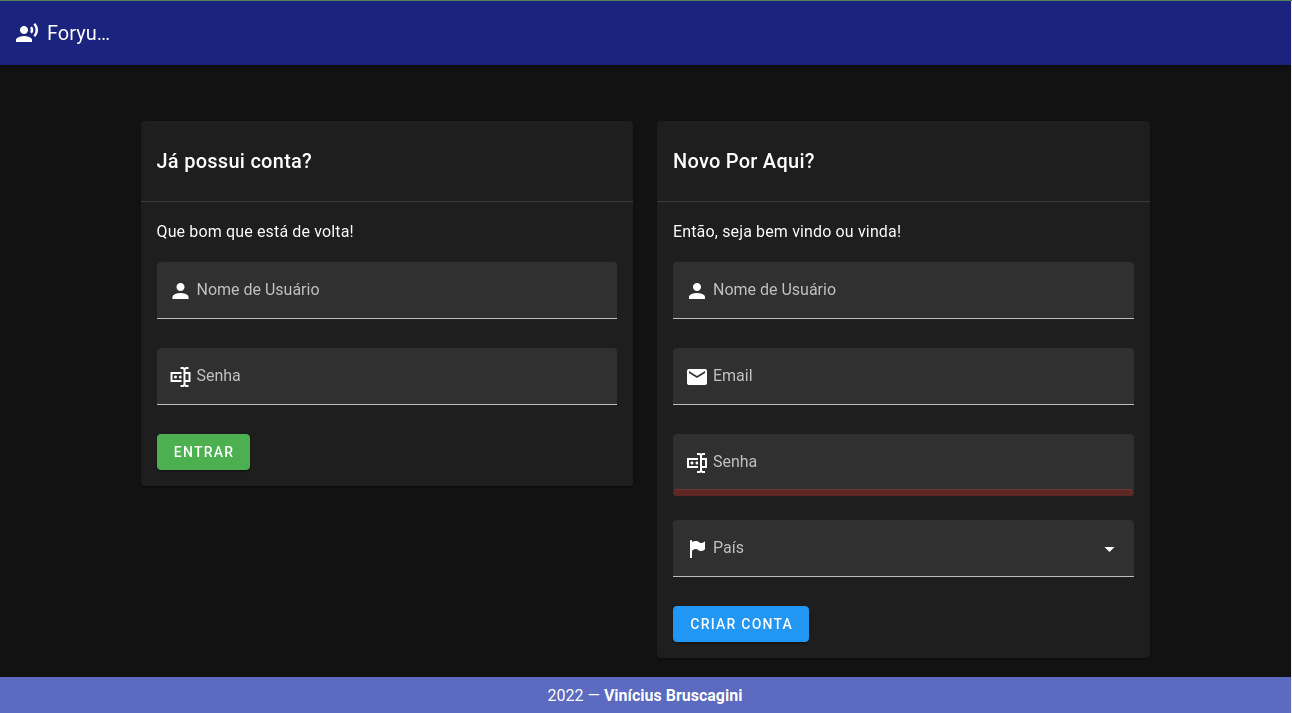
\includegraphics[width=1\textwidth]{prints/welcome.png}
    \caption{Tela de bem-vindo}\label{fig:welcome}
\end{figure}

\begin{figure}[H]
    \centering
    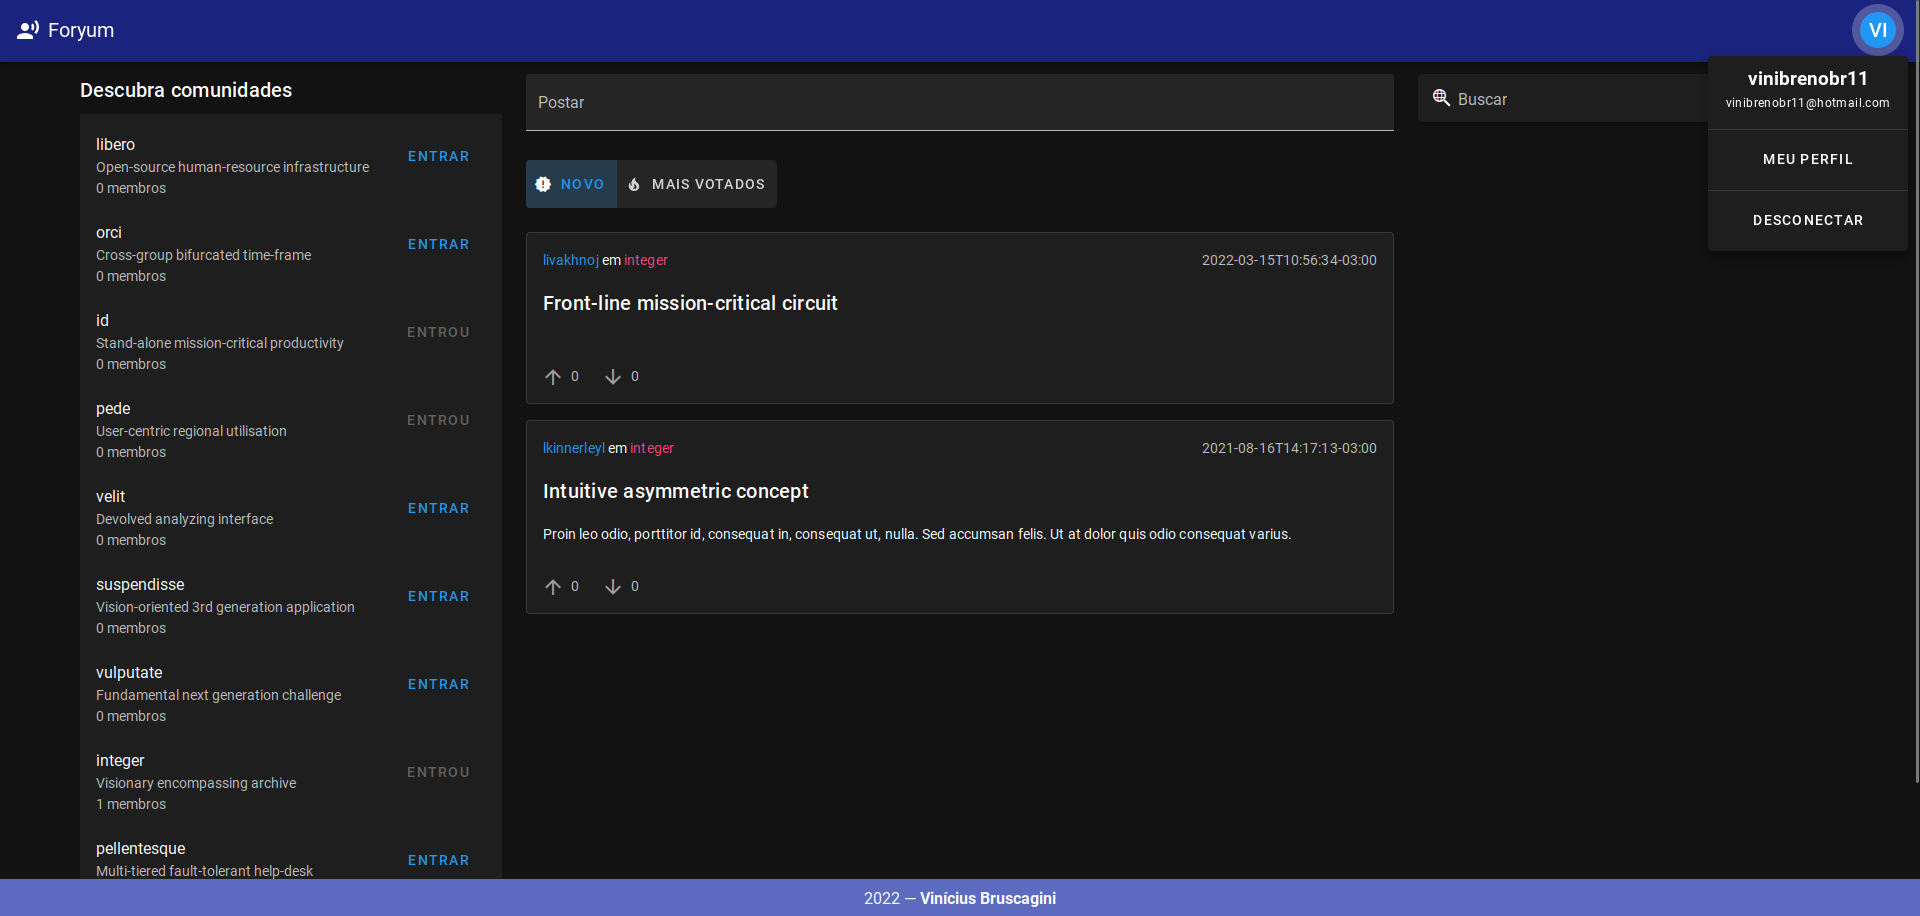
\includegraphics[width=1\textwidth]{prints/home.png}
    \caption{Tela \textit{home}}\label{fig:home}
\end{figure}

% Falar sobre a API, talvez colocar swagger aqui?
O Desenvolvimento da API em .NET foi finalizadada e todas as funcionalidades
usadas pela aplicação Web foram implementadas com restrições de acesso e esquemas de
segurança, um \textit{print} dos endpoints disponíveis nessa API é exibido
na figura~\ref{fig:swagger} através da biblioteca Swagger

\begin{figure}[H]
    \centering
    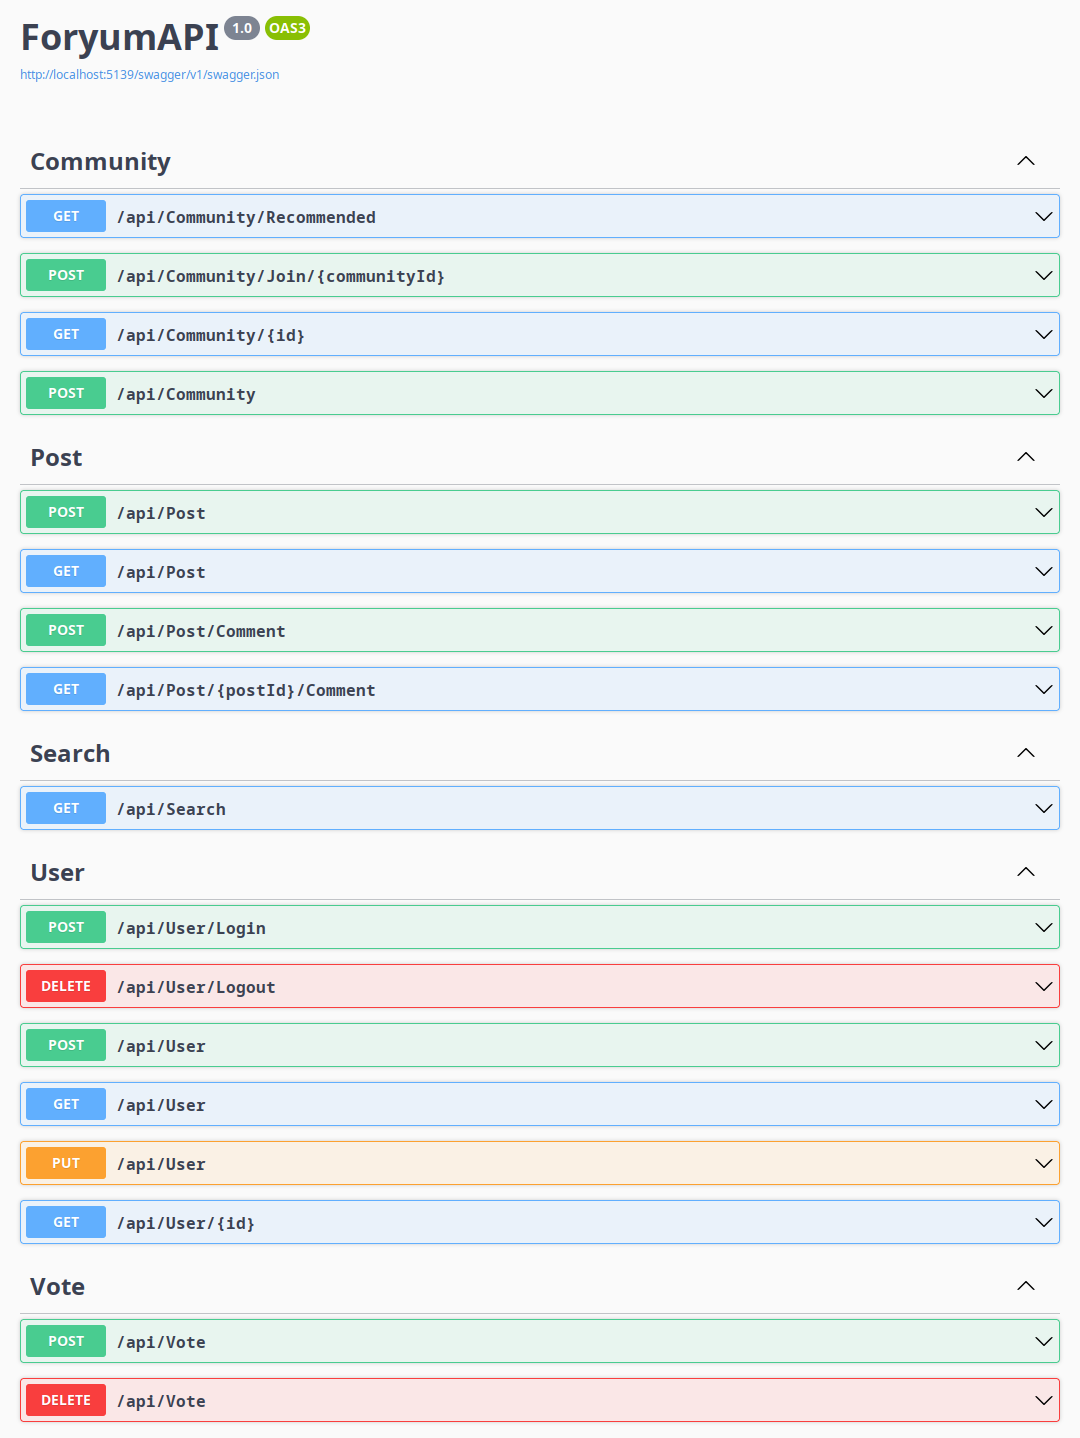
\includegraphics[width=1\textwidth]{prints/swagger.png}
    \caption{Print da tela do Swagger}\label{fig:swagger}
\end{figure}

\hl{Escrever sobre a documentacao e melhorar texto sobre a implementacao}

\section{Conclusão}

O artigo mostrou problemas existentes no ensino de desenvolvimento de software e propôs
a criação de um sistema com uma documentação abrangente para ajudar estudandes sobre alguns dos
conceitos e tecnologias usadas no desenvolvimento de software, além de prover uma abordagem prática
sobre o assunto. O Desenvolvimento e a criação da documentação do Software proposto está
quase sendo finalizado e todo esse material está disponível na plataforma \textit{GitHub}
para que estudantes do Curso do ADS e outros estudantes interessados possam usufruir e adiquirir
conhecimentos através desse material.

\bibliography{bibliografia}

\end{document}
